
%-----------------------------------------------------------------------------
%	PACKAGES AND THEMES
%-----------------------------------------------------------------------------
\documentclass[ignorenonframetext]{beamer}


\usepackage[beamer]{shortcut}
\graphicspath{{../../figures/}}

\tikzstyle{HEAD}=[fill=darkred!30,ultra thick]
\tikzstyle{highlight}=[fill=darkred!30]
\tikzset{onslide/.code args={<#1>#2}{%
  \only<#1>{\pgfkeysalso{#2}} % \pgfkeysalso doesn't change the path
}}

%-----------------------------------------------------------------------------
%	CUSTOM COMANDS
%-----------------------------------------------------------------------------

\def\keypoint#1{\hfill\textcolor{gray}{#1}}
\def\mycite#1{\keypoint{\cite{#1}}}

\def\extraLogo{}


%-----------------------------------------------------------------------------
%	PRESENTATION INFO
%-----------------------------------------------------------------------------

\title{A short intro to git}

% Presentation info
\author{Thomas Moreau} % Your name
\institute[CMLA]{ENS Paris-Saclay - CMLA} 
\date{15/8/25} % Date, can be changed to a custom date

% Custom footline
\event{MLMDA - PhD Kindergarden}
\location{Cachan, FRANCE}

% Setup the title style
\setbeamertemplate{title page}[frame]
\setlength\SizeTitleBox{.7\textwidth}

%-----------------------------------------------------------------------------
%	DOCUMENT
%-----------------------------------------------------------------------------

%% Title page
\begin{document} 

{
\setbeamertemplate{footline}{} 
\begin{frame}[t,plain]
\titlepage 
\end{frame}
}

	
	
\end{frame}


\begin{frame}{The goal of git...}

\textbf{Keeping track of a repository history:}
\begin{itemize}
	\itemsep.5em
	\item Versioning?? Why bother?
	\item Making archive of the full repo:\\
	Create a \code{zip} archive at fixed interval. This can become big.
	\item \textbf{Git!}
\end{itemize}
\vskip1em
\textbf{Sharing code with co-workers:}
\begin{itemize}
	\itemsep.5em
	\item Email changed files
	\item Dropbox-like synchronization
	\item \textbf{Git!}
\end{itemize}

\vskip1em
\centering
\visible<2>{\Large Git is a tool to keep track of history and share code.}
\end{frame}



\begin{frame}{How does it work?}
	
	
	\Large
	\begin{itemize}\itemsep1em
	\item Base object in git is the \code{commit}~~~\tikz[baseline=-.5em]{ \node[circle, draw, fill=green!20] {a};}
	\item Identifier commit has a hash \code{a : "baef63472"}.
	\item Git is base on a history tree notion.\\
		  Each commit is linked to its parent.\\[1em]
	\centering
	\tikz[]{
		\node[circle, draw, fill=blue!20] (0, 0) (a) {};
		\node[circle, draw, fill=blue!20, right=1em of a] (b) {};
		\node[circle, draw, fill=blue!20, right=1em of b] (c) {};
		\node[circle, draw, fill=blue!20, right=1em of c] (d) {};
		\node[circle, draw, fill=blue!20, right=1em of d] (e) {};
		\node[circle, draw, fill=blue!20, right=1em of e] (f) {};
		\node[circle, draw, fill=blue!20, right=1em of f] (g) {};
		\node[circle, draw, fill=green!20, below=1em of c] (c1) {};
		\node[circle, draw, fill=green!20, right=1em of c1] (d1) {};
		\node[circle, draw, fill=red!20, right=3em of d1] (e1) {};
		\node[circle, draw, fill=red!20, right=1em of e1] (f1) {};
		\draw[-] (a) -- (b) -- (c) -- (d) -- (e) -- (f) -- (g);
		\draw[-] (b) -- (c1) -- (d1) -- (e) --(e1) -- (f1);
		\node[rectangle, above=.5em of g] (virtual) {};
		\node[rectangle, right=1em of virtual] (note) {master};
		\draw[->, thick, shorten >=0.5em] (note) -- (g);
		\node[rectangle, below=.1em of f1] (virtual) {};
		\node[rectangle, right=1.5em of virtual] (note) {dev};
		\draw[->, thick, shorten >=0.5em] (note) -- (f1);
		\node[rectangle, below=.5em of d1] (virtual) {};
		\node[rectangle, right=1.5em of virtual] (note) {fix};
		\draw[->, thick, shorten >=0.5em] (note) -- (d1);
	}
\end{itemize}
3 branches: \{master; fix; dev\}

\end{frame}

\begin{frame}{What is a commit?}
\Large
	
	Keep track of code changes with its parent by comparing lines:\\[1em]
	{\centering
		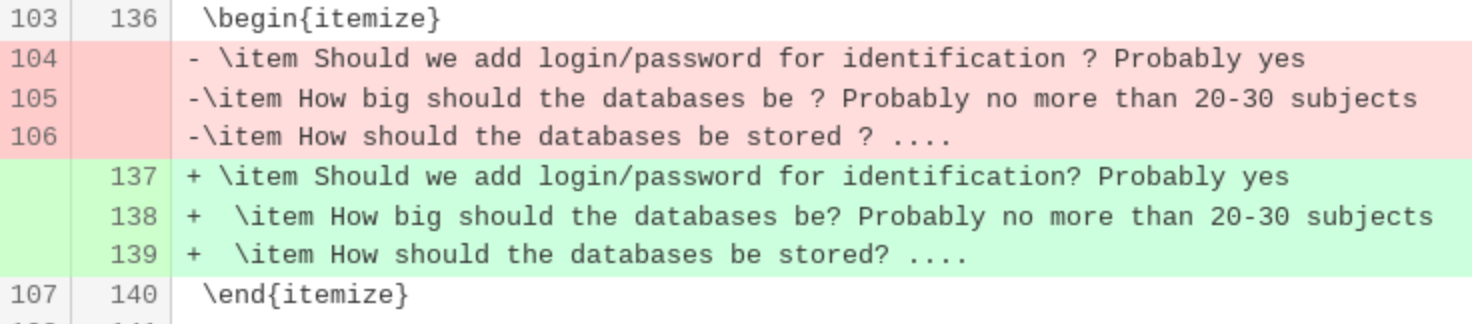
\includegraphics[width=\textwidth]{diff.png}
	}
	
	This is called a \code{diff}. The diff between the current state and the last commit is given by\\[.5em]
	\hskip2em\code{\$ git diff}
\end{frame}



\begin{frame}{Git diff}

	\Large
	The \code{git diff} command permits to access the differences between 2 commits.\\[1em]
	
	\begin{itemize}\itemsep1em
	\item \code{(dev)\$ git diff 1ab12f3e c837f6b5e}
	\item \code{(dev)\$ git diff master dev}
	\item \code{(dev)\$ git diff master}
\end{itemize}
\end{frame}

\begin{frame}{Creating a new commit}

	\Large
	\code{git status}: show the current state of a repo.\\
	~~~{\large Modified file; Ignored files; Staged files; conflicts....}

	\vskip.7em
	The command \code{git add} permits to prepare a commit:
	\begin{itemize}
		\item \code{(dev)\$ git add \$FILE1 \$FILE2 ...}
		\item \code{(dev)\$ git add -u}: Add all files modified
	\end{itemize}
	
	\vskip.7em
	The command \code{git commit} permits to create a commit.\\
	~~~{\large Composed of a message; put at the end of the current branch!}\\[.5em]
	\centering
	\tikz[]{
		\node[circle, draw, fill=blue!20] (0, 0) (a) {};
		\node[circle, draw, fill=blue!20, right=1em of a] (b) {};
		\node[circle, draw, fill=blue!20, right=1em of b] (c) {};
		\node[circle, draw, fill=blue!20, right=1em of c] (d) {};
		\node[circle, draw, fill=blue!20, right=1em of d] (e) {};
		\node[circle, draw, fill=blue!20, right=1em of e] (f) {};
		\node[circle, draw, fill=blue!20, right=1em of f] (g) {};
		\node[circle, draw, fill=green!20, below=1em of c] (c1) {};
		\node[circle, draw, fill=green!20, right=1em of c1] (d1) {};
		\node[circle, draw, fill=red!20, right=3em of d1] (e1) {};
		\node[circle, draw, fill=red!20, right=1em of e1] (f1) {};
		\node[circle, draw, thick, right=1em of f1, pattern=north west lines] (g1) {};
		\draw[-] (a) -- (b) -- (c) -- (d) -- (e) -- (f) -- (g);
		\draw[-] (b) -- (c1) -- (d1) -- (e) --(e1) -- (f1) --(g1);
	}
\end{frame}


\begin{frame}{Remotes}
	\Large
	Communication with the server:\\[1em]
	\begin{itemize}\itemsep1em
		\item \emph{HTTPS}: remote appears as \code{https://reine.cmla.ens-cachan.fr/user/repo}
		\item \emph{SSH}: remote appears as \code{git@reine.cmla.ens-cachan.fr:user/repo}
	\end{itemize}
	\vskip2em
	To see the available remotes: \code{git remote -v}
\end{frame}

\begin{frame}{Ssh disgression}
\Large
	\begin{itemize}\itemsep2em
		\item Secured communication protocole based on keys:\\
		Need to generate a key to communicate!
		\item Default use the port 22, CMLA use port 2333:\\
		Need configuration to access outside!
	\end{itemize}
	\vskip2em
	See \url{https://reine.cmla.ens-cachan.fr/mldma/presentation_git/wikis/git_setup}
\end{frame}

\begin{frame}{Interacting with a server (remote)}

	\Large
	Git is a distributed system. Each \code{remote} store the history tree.\\[1em]

	{\bf\centering There is a need for synchronization steps!}\\[1em]
	\only<-2>{
	\code{(dev)\$ git push}\\[2em]
		\tikz[]{
		\node[circle, draw, fill=blue!20] (0, 0) (a) {};
		\node[circle, draw, fill=blue!20, right=1em of a] (b) {};
		\node[circle, draw, fill=blue!20, right=1em of b] (c) {};
		\node[circle, draw, fill=blue!20, right=1em of c] (d) {};
		\node[circle, draw, fill=blue!20, right=1em of d] (e) {};
		\node[circle, draw, fill=blue!20, right=1em of e] (f) {};
		\node[circle, draw, fill=blue!20, right=1em of f] (g) {};
		\node[circle, draw, thick, right=1em of g, onslide=<1>{pattern=north west lines},
			  onslide=<2->{fill=blue!20}] (h) {};
		\draw[-] (a) -- (b) -- (c) -- (d) -- (e) -- (f) -- (g) -- (h);
		\node[rectangle, above=.5em of h] (virtual) {};
		\node[rectangle, right=1em of virtual] (note) {master};
		\draw[->, thick, shorten >=0.5em] (note.west) -- (h);
		\node[rectangle, below=1em of h] (virtual) {};
		\node[rectangle, right=1.5em of virtual] (note) {origin/master};
	\only<1>{
		\draw[->, thick, shorten >=0.5em] (note.west) -- (g);}
		\only<2>{
		\draw[->, thick, shorten >=0.5em] (note.west) -- (h);}
	}
	}
	\only<3->{
	\code{(master)\$ git pull}\\[2em]
	}
	\only<3>{
		\tikz[]{
		\node[circle, draw, fill=blue!20] (0, 0) (a) {};
		\node[circle, draw, fill=blue!20, right=1em of a] (b) {};
		\node[circle, draw, fill=blue!20, right=1em of b] (c) {};
		\node[circle, draw, fill=blue!20, right=1em of c] (d) {};
		\node[circle, draw, fill=blue!20, right=1em of d] (e) {};
		\node[circle, draw, fill=red!20, right=3em of d1] (e1) {};
		\node[circle, draw, fill=red!20, right=1em of e1] (f1) {};
		\draw[-] (a) -- (b) -- (c) -- (d) -- (e);
		\draw[-] (e) --(e1) -- (f1);
		\node[rectangle, above=.5em of e] (virtual) {};
		\node[rectangle, right=1em of virtual] (note) {master};
		\draw[->, thick, shorten >=0.5em] (note) -- (e);
		\node[rectangle, below=.1em of f1] (virtual) {};
		\node[rectangle, right=1.5em of virtual] (note) {origin/master};
		\draw[->, thick, shorten >=0.5em] (note) -- (f1);
	}
	}
	\only<4->{
		\tikz[]{
		\node[circle, draw, fill=blue!20] (0, 0) (a) {};
		\node[circle, draw, fill=blue!20, right=1em of a] (b) {};
		\node[circle, draw, fill=blue!20, right=1em of b] (c) {};
		\node[circle, draw, fill=blue!20, right=1em of c] (d) {};
		\node[circle, draw, fill=blue!20, right=1em of d] (e) {};
		\node[circle, draw, preaction={fill, red!20}, pattern=north west lines,
			  pattern color=blue!50, right=1em of e] (e1) {};
		\node[circle, draw, preaction={fill, red!20}, pattern=north west lines,
			  pattern color=blue!50, right=1em of e1] (f1) {};
		\draw[-] (a) -- (b) -- (c) -- (d) -- (e);
		\draw[-] (e) --(e1) -- (f1);
		\only<4>{
		\node[rectangle, above=.5em of e] (virtual) {};
		\node[rectangle, right=1em of virtual] (note) {master};
		\draw[->, thick, shorten >=0.5em] (note) -- (e);
		}
		\only<5>{
		\node[rectangle, above=.5em of f1] (virtual) {};
		\node[rectangle, right=1em of virtual] (note) {master};
		\draw[->, thick, shorten >=0.5em] (note) -- (f1);
		}
		
		\node[rectangle, below=.1em of f1] (virtual) {};
		\node[rectangle, right=1.5em of virtual] (note) {origin/master};
		\draw[->, thick, shorten >=0.5em] (note) -- (f1);
	}
	}
\end{frame}

\begin{frame}{Extra concepts}
\Large
\begin{itemize}\itemsep1em
	\item Rebase
	\item Merge
	\item Conflicts
	\item \dots
\end{itemize}
\end{frame}

\begin{frame}{That's all folks!}
	\centering
	\Huge \textbf{Questions?}
\end{frame}



\end{document} 